\section{Browser Media}

A true distributed media streaming application must also rely on distributed content generation. Users of the system must be able to record media on their connected devices and provide a stream to the network. Other users must be able to consume those streams of audio and video data with their respective devices. Considering the constraint, that the application should be executable in a browser, used media formats have to meet further requirements.

\subsection{Media Pipeline}
\label{browser-api}

Modern browsers implement a set of JavaScript \glspl{api} that comply with the {\textit{Media Capture and Streams}} draft \cite{media-capture-and-streams} of the \gls{w3c}. The draft defines an interface for media streams that can contain multiple tracks, which in turn can contain multiple channels. In its most common configuration a stream would consist of a video and audio track and the latter would contain two channels for a stereo signal. A media stream instance can either be created locally or originate from a network source. Either of those streams can be presented to the local user or streamed to a network connection. \cite{media-capture-and-streams} denominates these two usages as sources and sinks respectively.

\subsubsection{Stream Sources}

Streams can only be recorded locally after the application has acquired user consent from the browser and \gls{os}. The user media \gls{api} allows to constrain recording parameters, such as video resolution, frame rate or audio volume (see \ref{lst:recording-constraints}). The satisfiability of these constraints however, depends on browser, \gls{os} and device compatibility.

\begin{Listing}
\begin{lstlisting}
{
  "audio": {
    "autoGainControl": false,
    "channelCount": 2,
    "echoCancellation": true,
    "volume": {
      "ideal": 0.75
    }
  },
  "video": {
    "facingMode": {
      "exact": "user"
    },
    "frameRate": {
      "ideal": 60
    }
  }
}
\end{lstlisting}
\caption{Example media stream recording constraints for the getUserMedia API}
\label{lst:recording-constraints}
\end{Listing}

A media stream can also originate from a network source. \Gls{http} streaming and \gls{webrtc} connections are the two common approaches. The former shall be further discussed in section~\ref{subsec:http-streaming}, the latter in section~\ref{subsec:webrtc-media}.

\subsubsection{Stream Sinks}

The browser media pipeline provides that a stream ends with a so called sink. To display it to the local user, the \gls{html} standard \cite[\S4.7]{html-w3c} defines media tags such as \lstinline|<audio>| and \lstinline|<video>|. These tags feature a JavaScript \gls{api} for themselves to control playback and react to stream changes. A stream can be directly attached to the elements and the browser handles low-level playback features such as pre-loading, buffering and random access. To forward the stream to a remote system, a media stream can also be directed to an outgoing \gls{webrtc} connection. The \gls{api} of which states the browser should handle stream constrain negotiation like letting sender and receiver agree on a video resolution \cite[\S5.1]{webrtc-w3c}.

\subsubsection{Media Source Extensions}

In 2016 the \gls{w3c} enhanced the capabilities of browser media pipelines by introducing the \gls{mse} standard. With this extension, a JavaScript application can dynamically adapt an audio or video stream. According to \cite{mse-google}, the main use cases are adaptive streaming, dynamic ad insertion and time shifting. As an alternative to a media stream, the \gls{mse} standard introduces a media source and a source buffer API to the JavaScript media pipeline. A media source can be directly assigned to an \lstinline|<audio>| or \lstinline|<video>| tag and contains a set of source buffers. These buffers can then be filled, sought and flushed to allow seamless playback from multiple stream sources. The \gls{mse} itself does not enforce any kind of codec to promote inter device and browser compatibility.

\begin{figure}
\centering
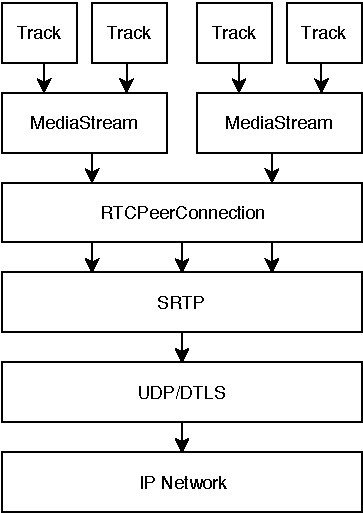
\includegraphics[width=.5\textwidth]{graphics/media-stream-pipeline.pdf}
\caption{Browser media streaming pipeline and network stack}
\label{fig:pipeline}
\end{figure}

\subsection{WebRTC Media}
\label{subsec:webrtc-media}

"WebRTC provides media acquisition and delivery as a fully managed service: from camera to the network, and from network to the screen", as Ilya Grigorik describes it \cite[\S18.5]{high-performance-browser-networking}. So, for streaming media from one peer to another, the browser provides a powerful, high-level interface to developers. An \lstinline|RTCPeerConnection| as defined by \cite[\S4.4]{webrtc-w3c} can add streams on the producer side as well as receive streams on the consumer side. Under the hood, however, browsers must perform a complex transmission process (see \cref{fig:pipeline}). Because \gls{webrtc} runs on top of \gls{udp}, the connection is inherently unreliable. However, for live streaming applications, timeliness at the cost of video quality is deemed more important than a persistent quality at the cost of delays and stutter \cite[\S18.3]{high-performance-browser-networking}. The \gls{webrtc} network engine uses a stack of two transport protocols to deliver the best possible media stream across a constantly changing connection. \Gls{srtcp} is used to measure and exchange package loss, sequence errors, jitter and more between the two peers. Those statistics influence how the browser chooses appropriate quality and codec settings. \gls{srtp} on the other hand is used to transmit the actual audio and video streaming data.

\subsection{HTTP Streaming}
\label{subsec:http-streaming}

With the adoption of \gls{html} 5, online video streaming has moved from plugin-based approaches like Adobe Flash \cite{adobe-flash} or Microsoft Silverlight \cite{microsoft-silverlight} to native, browser-based technologies. Namely, two competitors have emerged: \gls{hls} and \gls{mpeg-dash}. The former was developed by Apple, and although not being internationally standardized, \gls{hls} was adopted by some other vendors as well \cite{caniuse-hls}. The successor \gls{mpeg-dash}, was adopted as a standard \cite{iso-mpeg-dash}, does not require specific video codecs and has built-in \gls{drm} capabilities. What both have in common, is that they split media streams into short segments and use a manifest file to stitch them back together on the client side. This, plus the fact that they run on top of HTTP, make them work well on modern \glspl{cdn}, as \cite{hls-vs-dash} points out.

\subsection{Media Formats}

When considering the fragmented landscape of browser media streaming technologies, the actual media encodings being used are even more vendor and version dependent, as the compatibility table for in-browser playback at \cite{media-format-browser-compat} shows. For playback, common ground between vendors can be found with VP8 compression in a WebM container or H.264 in MP4. However, when trying to encode media recorded on-device, the set of supported formats is even smaller and, according to Phillips, the broadest interoperability can be achieved with H.264 \cite[\S5.1]{webrtc-hacks-safari}. On the audio side, more modern and effiecient formats like Opus and Vorbis have emerged. However, the widest support is still enjoyed by traditional MP3 \cite{media-format-browser-compat}.

\subsection{Video Streaming Applications}

Efficiently delivering streaming video over the internet has long been an active research topic. Non-linearity, rich user interactions and diversification of media sources have driven users from consuming terrestrial television or hard copy video to internet based media platforms.
These platforms and their underlying technologies can be categorised by (1) offered media types and (2) content distribution architecture. Some platforms offer pre-produced videos, be it professional movies or amateur vlogs, to be streamed on demand (TODO: Video-on-demand). Other platforms offer live video streams with realtime viewer interactions.
Both type of video offerings can be found to be built upon a centralised or decentralised streaming architecture. Figure X shows examples of platforms arranged by category.

        on-demand       live
central youtube         periscope         
        netflix         twitch
        tiktok
pee2pee zatoo           appear.in
        popcorn         <mitosis>
Figure X

\subsection{Centralised Streaming}

- server and transcoding cost
- scaling up
- censorship

\subsection{Decentralised Streaming}

- content discovery
- overlay creation, timetofirstbyte
- ...problems of streamer cite

\section{User-generated Streaming Applications}

~Although distributed video streaming technologies have been around for a while \cite{TODO}, today's major platforms for user-generated live streaming build upon centralised delivery architectures \cite{periscope, twitch, facebook-live}.~

According to \citet{twitch-case} these platforms are characterised by opening content creation to all of their users and allowing video consumers to give realtime feedback in the form of chats or likes.

- periscope

twitch
- paid transcoding \cite[\S2]{twitch-study}
- transcoding latency of 10seconds \cite[\S4.2]{twitch-study}
